% !TeX root = ../../thesis.tex

\chapter{Evaluation}
\label{chp:evaluation}


In this chapter the designed hardware and software will be evaluated, for both the DC and the AC testbeds.
After that, simulation will evaluate the scalability of the setups.


As explained in \autoref{sec:interference-solution}, the correctional data that is calculated is compared to a threshold.
This data can be less than or equal to the threshold or it can be greater than the threshold.
For each of these cases, the data can also be correct or wrong.
So there are four categories to consider:


\begin{itemize}

	\item True Positive: The correlation is above the threshold, meaning the sequence is present in the signal according to the receiver and the transmitter actually did send this sequence.

	\item False Positive: The correlation is above the threshold, meaning the sequence is present in the signal according to the receiver but the transmitter did not send this sequence and due to interference from other sequences the correlation became higher than the set threshold.

	\item True Negative: The correlation is not above the threshold, meaning the sequence is not present in the signal according to the receiver and the transmitter did not send this sequence.

	\item False Negative: The correlation is not above the threshold, meaning the sequence is not present in the signal according to the receiver but the transmitter did send this sequence and due to interference from other sequences the correlation became lower than the set threshold.


\end{itemize}




When there is a system for which we can classify the results as false/true-positives and false/true-negatives, we can evaluate the system's performance by investigating the precision and recall.
The definitions of precision and recall can be found in \autoref{eq:precision} and \autoref{eq:recall} respectively, where $tp$ stands for the number of true-positives, $fp$ stand for the number of false-positives and $fn$ stand for the number of false-negatives.

\begin{equation}
	\label{eq:precision}
	\text{Precision } = \frac{tp}{tp + fp}
\end{equation}

\begin{equation}
	\label{eq:recall}
	\text{Recall } = \frac{tp}{tp + fn}
\end{equation}

This method provides two metrics to consider.
Ideally we want only one metric to consider and draw conclusion based on that.
We can take the weighted average of the two metrics.
This is called the F-measure \cite{sokolova2009systematic} and is the harmonic mean of the precision and recall.
The definition of the F-measure can be seen in \autoref{eq:F-measure}.

\begin{equation}
	\label{eq:F-measure}
	F = 2 \times \frac{\text{precision} \times \text{recall}}{\text{precision} + \text{recall}}
\end{equation}






% !TeX root = ../../../thesis.tex

\section{Hardware}
\label{sec:hardware-evaluation}

The following two sections will describe the evaluation of the designed hardware and software, first for the DC testbed and then the AC testbed.
All LEDs will be assigned an ID that has the same length.
As discussed in \autoref{chp:cdma}, the correlation calculations only hold when CDMA codes are used from the same set.
The ID is programmed in the micro-controller.% before they are installed in their position in a room.
Based on the length of this ID, a certain amount of LEDs are supported, which is explained in \autoref{sec:interference-solution}.
But when the number of lights in the building increases, the new total number of lights may exceed the number of IDs.
When this happens all the IDs must be changed to another ID of a different length that does support the new amount of lights.
This may be done via a photo-diode as a receiver for each light, to receive the new ID.
In this way each light can be used again, even when the total number of lights increases.


In the following evaluation sections, all attached LEDs will be modulating with a different ID per LED.
This represents the worst case: Every LED is modulating and thereby causing interference.
Since every LED will be modulating we can evaluate if the state of the LEDs can indeed be identified as being on.
If this is not the case, this will be classified as a false-negative.
But for completeness we must also evaluate what happens when the system tries to identify an ID which corresponds to an LED that is off.
For this reason, an extra ID will be used to represent an LED in an off state.
The raw ADC signal will be showed as well as the steps that are required in order to process the raw data such that the correlation calculations can be performed.
Next, the correlation graph will be showed for an ID that is being used to modulate one of the LEDs as well as the correlation graph for the extra ID which represents an LED in an off state. 
Finally the F-measure will be showed for these correlation graphs.









% !TeX root = ../../../../thesis.tex

\subsection{DC}
\label{subsec:dc-testbed-eval}

The DC testbed has six LEDs, as explained in \autoref{subsec:dc-testbed}.
Therefor six Gold codes will be used for the LEDs with a seventh code used to represent an LED in an off state.
From \autoref{tbl:correlation-gold-families}, we can see that for $m = 6$, where $m$ is the number of simultaneous transmitters such that no destructive interference takes place, requires a code length of 511 or higher.
With the DC testbed the experiments have been performed with a constant modulation frequency of 1 kHz.
Every two successive samples are $\frac{1}{1000} = 1$ ms apart.

In \autoref{fig:raw-dc-testbed-adc-data-n=9} the raw ADC from the DC testbed can be seen.
The left y-axis represents the raw ADC data and the right y-axis is converted to current.
Six LEDs are simultaneous continuously modulating with different starting times.
From the figure, seven horizontal lines can be seen.
Each line represents how many LEDs are on, none through six.
This raw data is already in a form for which we can start calculating the correlation with a Gold sequence, no additional signal processing is needed.

In \autoref{fig:correlation-dc-testbed-n=9}, the correlation for one Gold sequence can be seen, which is also one of the sequences used to modulate an LED and the correlation for the extra Gold sequence can be seen, which is not part of the sequences used to modulate any LED and represent the LED is an off state.
All the correlation results from the Gold code used to modulate and LED with, stay below the threshold (See \autoref{eq:T}) except for the noticeable peaks.
These peaks indicate that the LED is on, which in fact is the case.
These peaks occur when the correlation is calculated when there is no time shift as already shown in \autoref{fig:autocorr-gold}.
The correlation results from the extra code all stay below the threshold, meaning the LED represented by this code is off, which is that case.

Since all the correlation levels are below the threshold, and the peaks are above the threshold, every result is correct.
There are only true positives and true negatives.
So the F-measure is equal to $1$ according \autoref{eq:F-measure}.
This can also be seen in \autoref{fig:f-measure-dc-testbed-n=9}.

\begin{figure}[!tbp]
  \centering
  \begin{minipage}[b]{0.49\textwidth}
    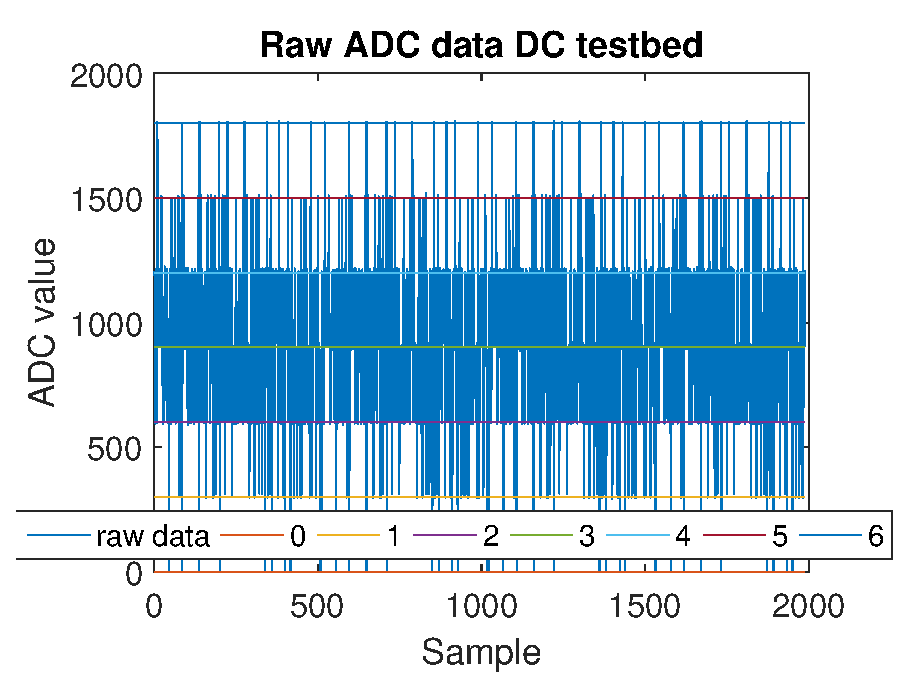
\includegraphics[width=\textwidth]{chapters/evaluation-chapters/hardware/dc/raw-dc-testbed-adc-data-n=9.eps}
    \caption{Raw ADC data from the DC testbed. With seven distinguishable entries, following the on-state of the combinations of LEDs. With a sequence length of 511.}
	\label{fig:raw-dc-testbed-adc-data-n=9}
  \end{minipage}
  \hfill
  \begin{minipage}[b]{0.49\textwidth}
    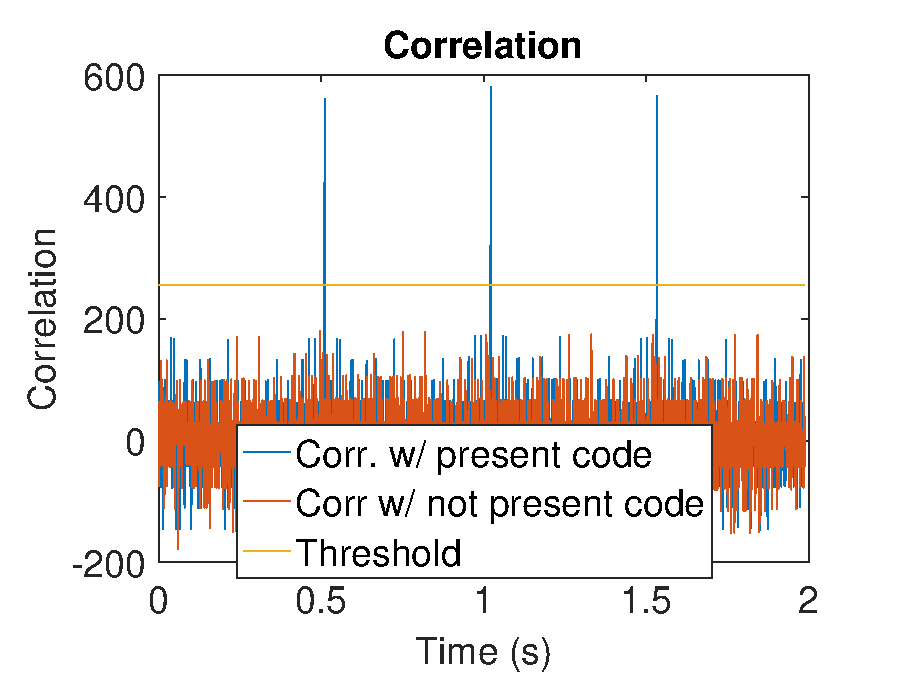
\includegraphics[width=\textwidth]{chapters/evaluation-chapters/hardware/dc/correlation-dc-testbed-n=9.eps}
    \caption{Correlations results from Gold sequences which are and which are not present, with the decision threshold. With a sequence length of 511.}
	\label{fig:correlation-dc-testbed-n=9}
  \end{minipage}
\end{figure}

To show how the F-measure would behave when there are false positives and/or false negatives a different Gold set is chosen.
A length of 127 is chosen, since it may only have three simultaneous continuously modulating LEDs (\autoref{tbl:correlation-gold-families}).
Again the six LEDs are simultaneous continuously modulating with different starting times.
For which the raw ADC can be seen in \autoref{fig:raw-dc-testbed-adc-data-n=7} on the left y-axis and on the right y-axis the current.
And the correlation can be found in \autoref{fig:correlation-dc-testbed-n=7}.
In the correlation figure, peaks can be seen that cross the threshold line, which are the autocorrelation peaks of the sequence.
They are supposed to be there.
But also other results can be seen to cross the threshold line.
These are the false positives, they occur because this code length can not support this much simultaneous transmitters.
The F-measure for these correlation results can be found in \autoref{fig:f-measure-dc-testbed-n=7}.


\begin{figure}[!tbp]
  \centering
  \begin{minipage}[b]{0.49\textwidth}
    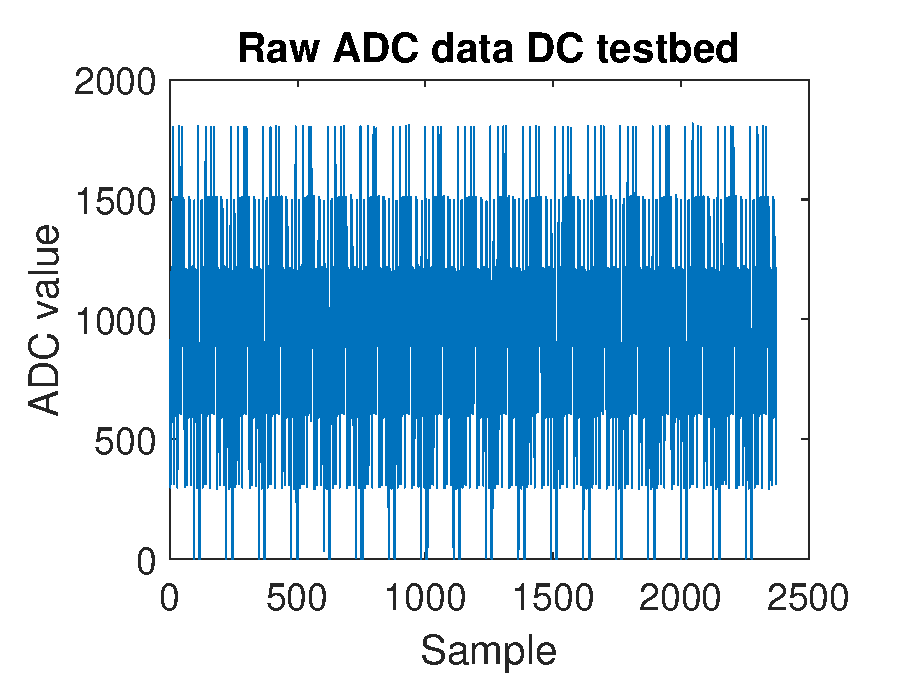
\includegraphics[width=\textwidth]{chapters/evaluation-chapters/hardware/dc/raw-dc-testbed-adc-data-n=7.eps}
    \caption{Raw ADC data from the DC testbed. With seven distinguishable entries, following the on-state of the combinations of LEDs. With a sequence length of 127  on the DC testbed.}
	\label{fig:raw-dc-testbed-adc-data-n=7}
  \end{minipage}
  \hfill
  \begin{minipage}[b]{0.49\textwidth}
    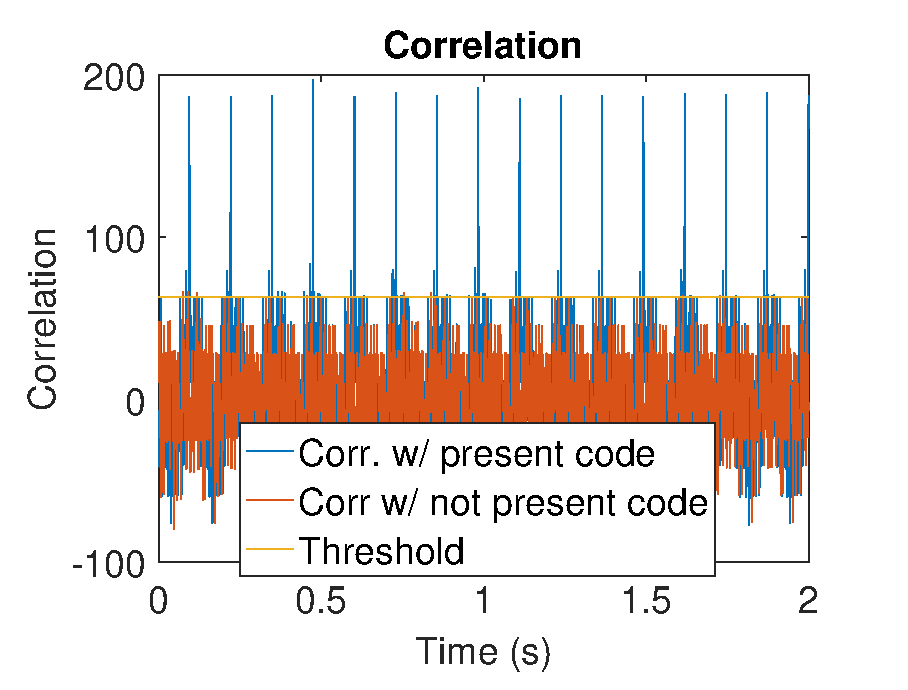
\includegraphics[width=\textwidth]{chapters/evaluation-chapters/hardware/dc/correlation-dc-testbed-n=7.eps}
    \caption{Correlations results from Gold sequences which are and which are not present, with the decision threshold. With a sequence length of 127 on the DC testbed.}
	\label{fig:correlation-dc-testbed-n=7}
  \end{minipage}
\end{figure}


\begin{figure}[!tbp]
  \centering
  \begin{minipage}[b]{0.49\textwidth}
    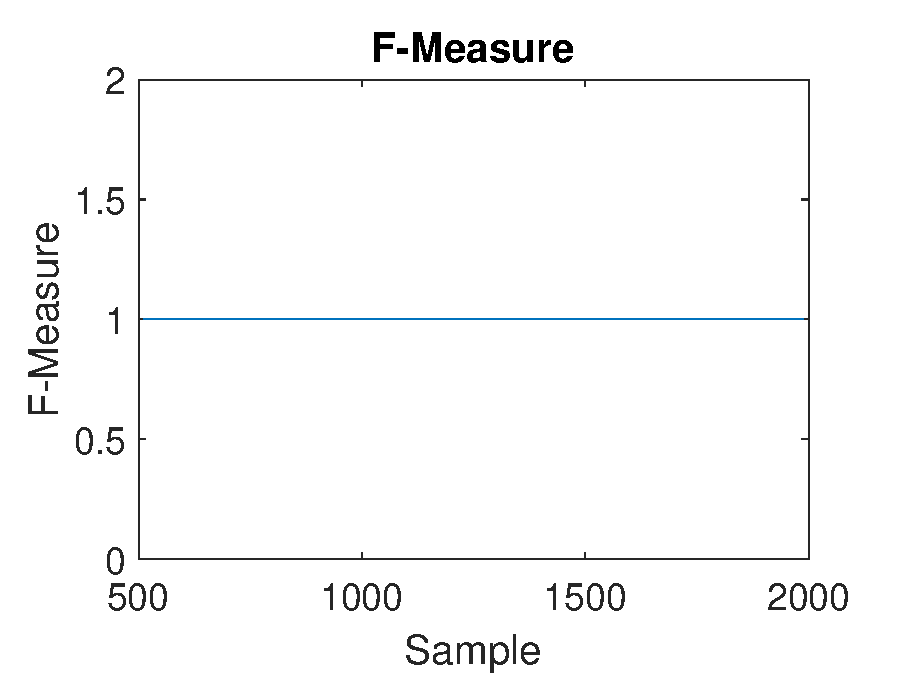
\includegraphics[width=\textwidth]{chapters/evaluation-chapters/hardware/dc/f-measure-dc-testbed-n=9.eps}
	\caption{F-Measure of DC testbed correlation (\autoref{fig:correlation-dc-testbed-n=9}), with sequence length of 511.}
	\label{fig:f-measure-dc-testbed-n=9}
  \end{minipage}
  \hfill
  \begin{minipage}[b]{0.49\textwidth}
	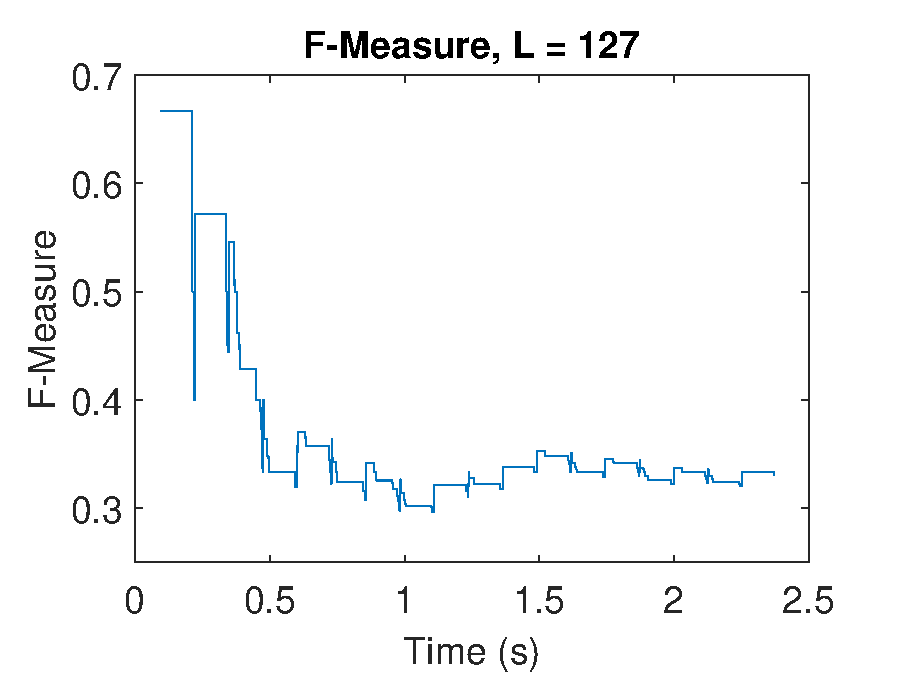
\includegraphics[width=\textwidth]{chapters/evaluation-chapters/hardware/dc/f-measure-dc-testbed-n=7.eps}
	\caption{F-Measure of DC testbed correlation (\autoref{fig:correlation-dc-testbed-n=7}), with sequence length of 127.}
	\label{fig:f-measure-dc-testbed-n=7}
  \end{minipage}
\end{figure}

% !TeX root = ../../../../thesis.tex

\subsection{AC}


The AC testbed has three LEDs, as explained in \autoref{subsec:ac-testbed}.
Therefor three Gold codes will be used.
From \autoref{tbl:correlation-gold-families}, we can see that for $m = 3$, the number of simultaneous transmitters such that no destructive interference takes place, requires a code length of 127 or higher.
With the AC testbed the experiments have been performed with a constant modulation frequency of 10 kHz.
Two successive samples are $\frac{1}{10000} = 0.1$ ms apart, except for when the triggering circuit detects that no modulation or sampling can take place anymore.
In that case the sampling and modulation is paused until the triggering circuit detects that modulation and sampling can take place again.


In \autoref{fig:raw-ac-testbed-adc-data} the incoming signals to the current sampler can be seen.
The raw data from the ADC can be seen as well as the output of the triggering circuit.
Also the mean of the ADC values are plotted for signal processing later on.
The large peaks that can be seen are the charging currents of the capacitor for the voltage sources as discussed in \autoref{subsubsec:non-disturbing-voltage-source}.

When only the signal is considered when the output from the triggering circuit is low, the charing peaks are all filtered out.
Next each sample is subtracted with the mean of all the samples and then the absolute value is taken.
Now we have the fully processed signal, ready to do correlation calculations with.
The processed signal can be seen in \autoref{fig:processed-ac-testbed-adc-data}.



\begin{figure}
  \centering
  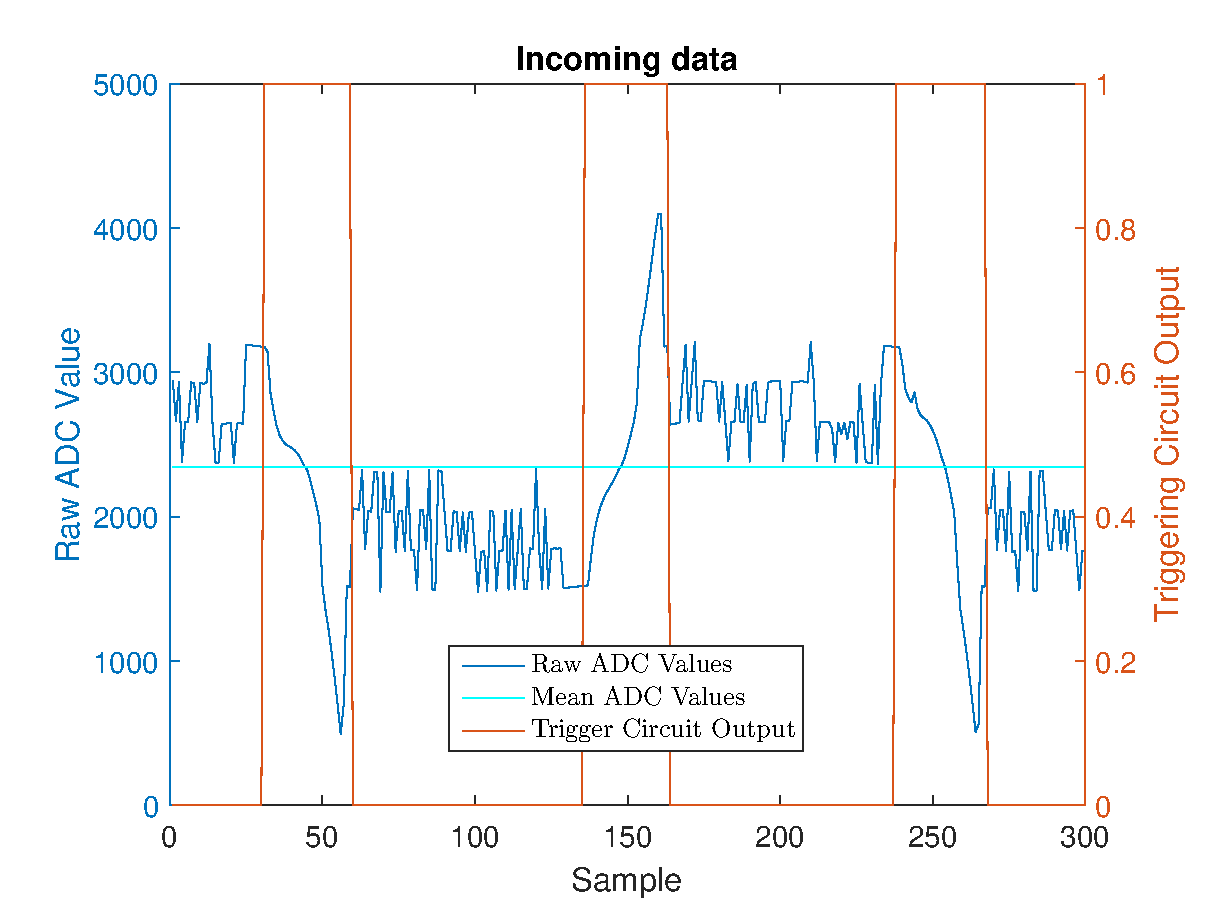
\includegraphics[width=0.8\textwidth]{chapters/evaluation-chapters/hardware/ac/raw-ac-testbed-adc-data.eps}
    \caption{Incoming data to the AC current sampler. The raw ADC values are plotted as well as the triggering circuit output. Also the mean of the raw ADC values is plotted. Gold sequence of length 127.}
  \label{fig:raw-ac-testbed-adc-data}
\end{figure}


\begin{figure}
  \centering
  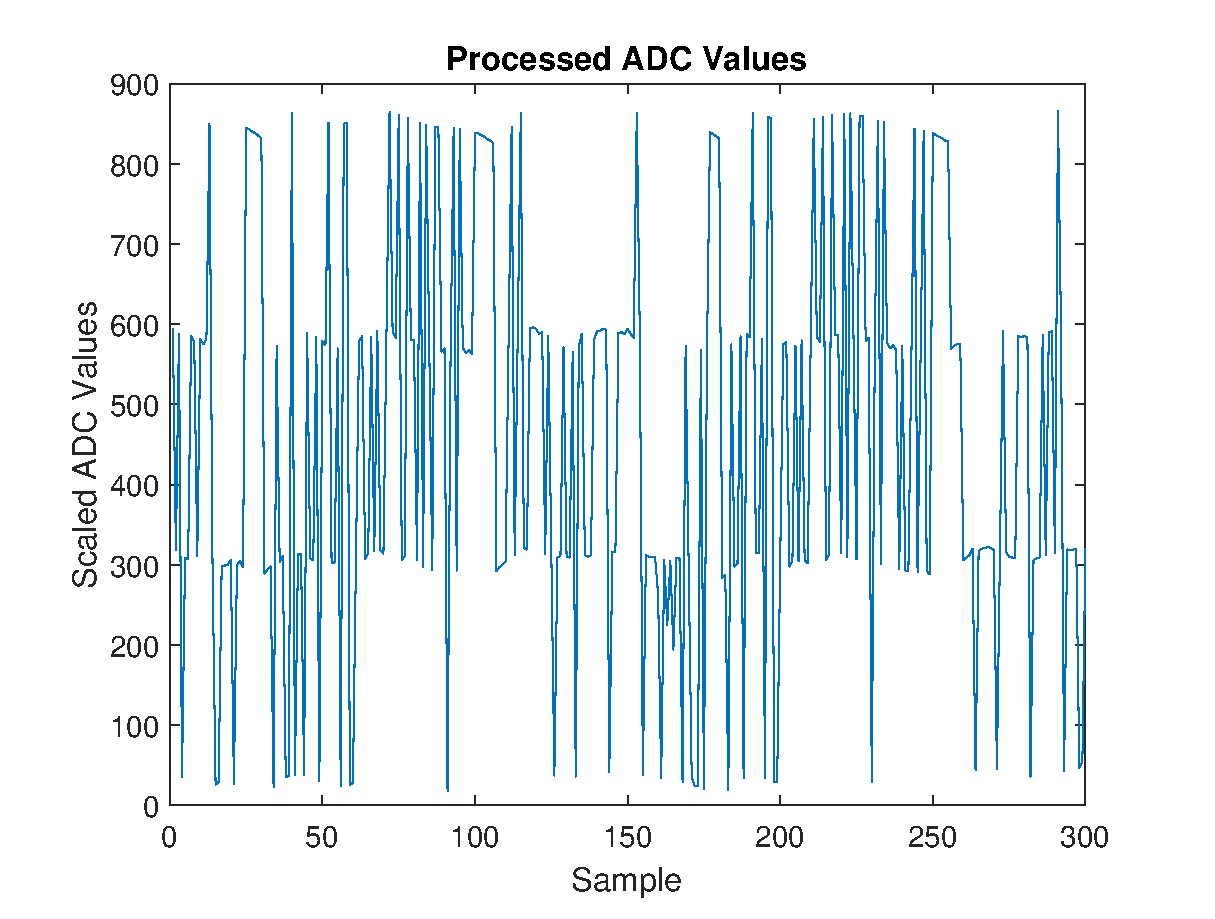
\includegraphics[width=0.8\textwidth]{chapters/evaluation-chapters/hardware/ac/processed-ac-testbed-adc-data.eps}
    \caption{Fully processed ADC values, where four distinguishable levels can be seen. With the on-state from zero to all three LEDs, on the AC testbed.}
  \label{fig:processed-ac-testbed-adc-data}
\end{figure}



%\begin{figure}[!tbp]
%  \centering
%  \begin{minipage}[b]{0.49\textwidth}
%    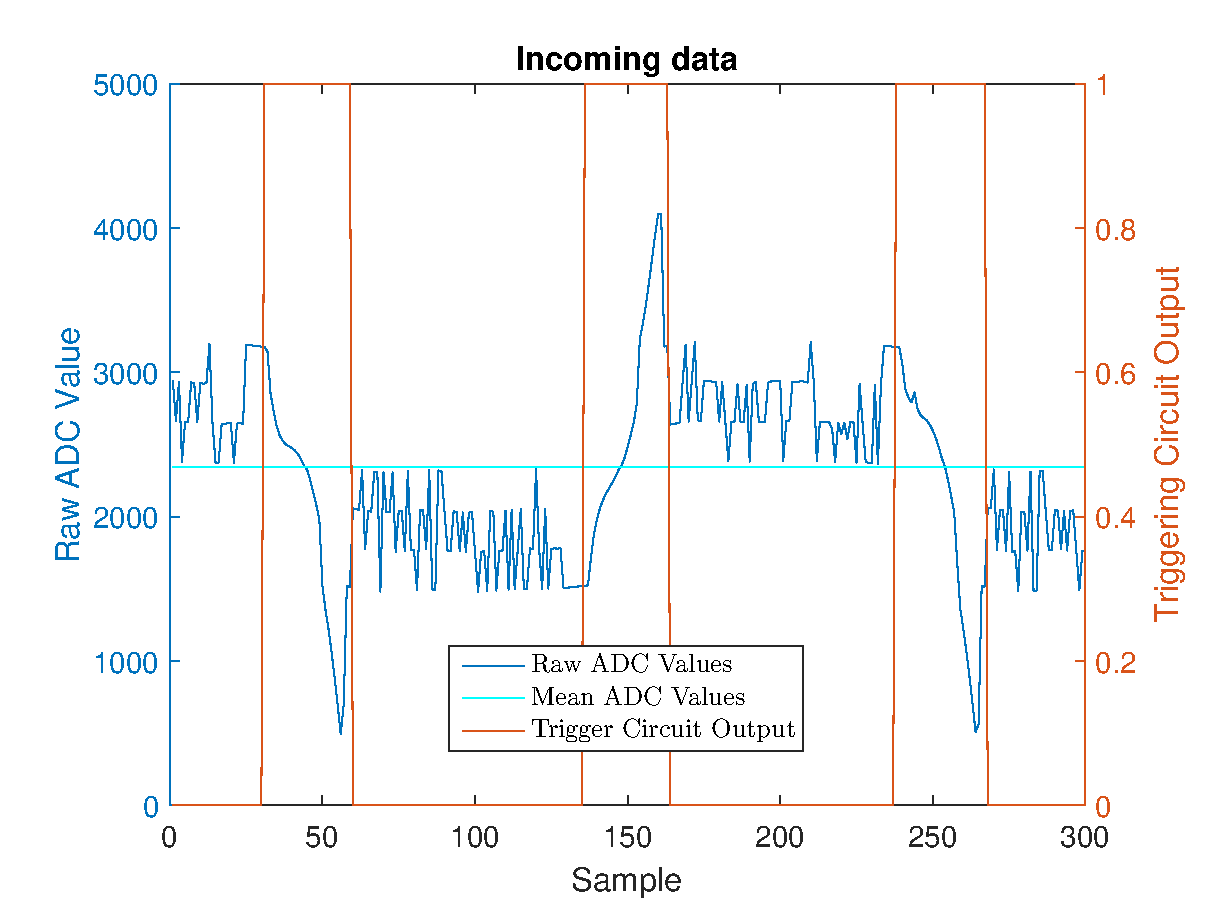
\includegraphics[width=\textwidth]{chapters/evaluation-chapters/hardware/ac/raw-ac-testbed-adc-data.eps}
%    \caption{Incoming data to the AC current sampler. The raw ADC values are plotted as well as the triggering circuit output. Also the mean of the raw ADC values is plotted. Gold sequence of length 127.}
%	\label{fig:raw-ac-testbed-adc-data}
%  \end{minipage}
%  \hfill
%  \begin{minipage}[b]{0.49\textwidth}
%    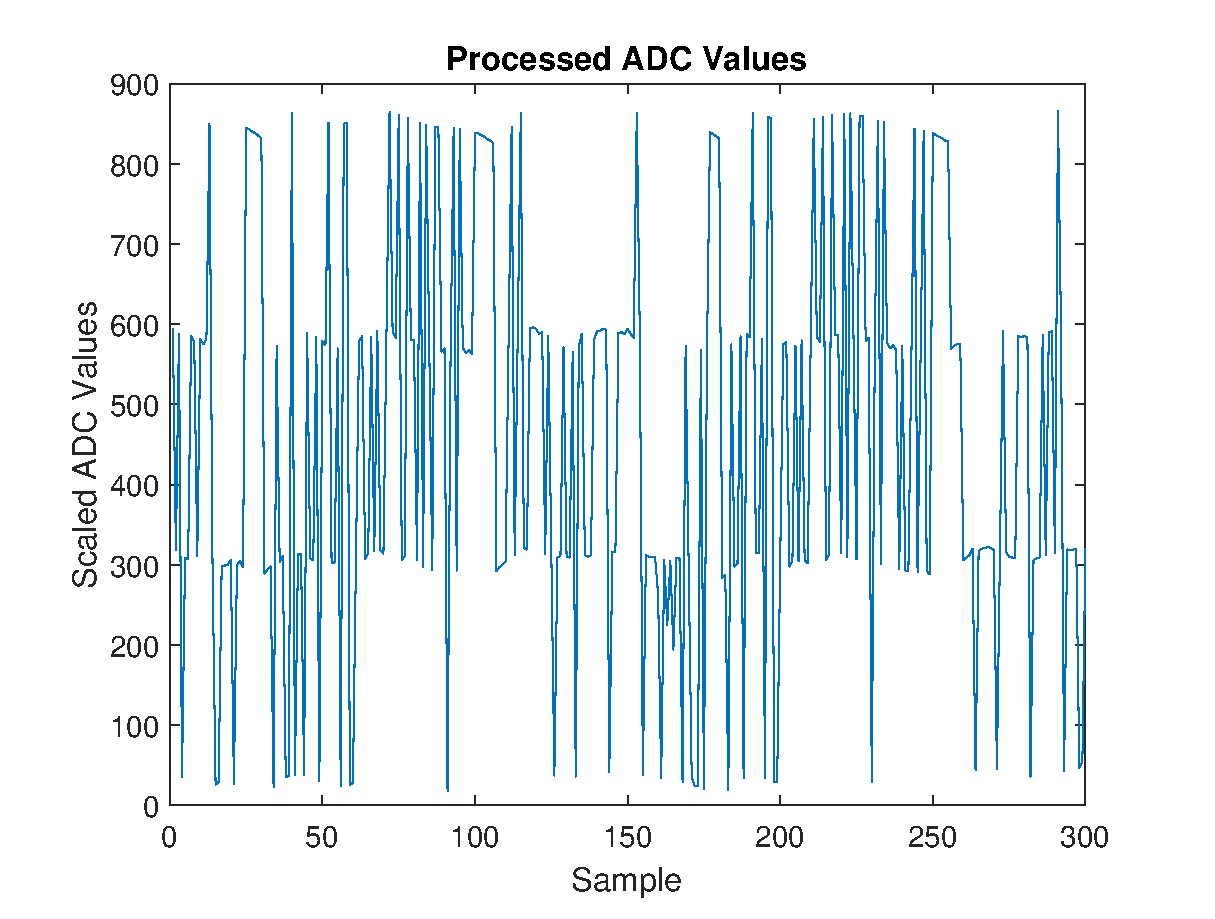
\includegraphics[width=\textwidth]{chapters/evaluation-chapters/hardware/ac/processed-ac-testbed-adc-data.eps}
%    \caption{Fully processed ADC values, where four distinguishable levels can be seen. With the on-state from zero to all three LEDs, on the AC testbed.}
%	\label{fig:processed-ac-testbed-adc-data}
%  \end{minipage}
%\end{figure}


In \autoref{fig:correlation-ac-testbed}, the correlation for one Gold sequence can be seen, which is also one of the sequences used to modulate an LED and the correlation for another Gold sequence can be seen, which is not part of the sequences used to modulate any LED.
All the correlation results stay below the threshold (See \autoref{eq:T}) except for the noticeable peaks.
These peaks occur when the correlation is calculated when there is no time shift as already shown in \autoref{fig:autocorr-gold}.

Since all the correlation levels are below the threshold, and the peaks are above the threshold, every result is correct.
There are only true positives and true negatives.
So the F-measure is equal to $1$ according \autoref{eq:F-measure}.

\begin{figure}[htb]
	\centering
	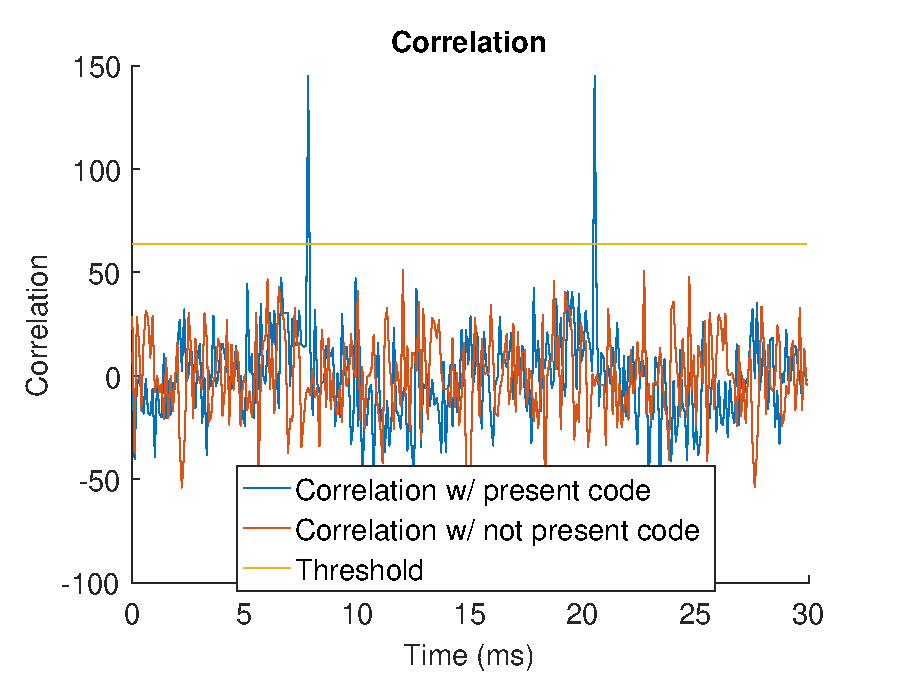
\includegraphics[angle=0,width=\textwidth,keepaspectratio]{chapters/evaluation-chapters/hardware/ac/correlation-ac-testbed.eps}
	\caption{Correlations results from Gold sequences which are and which are not present, with the decision threshold. With a sequence length of 127 on the AC testbed.}
	\label{fig:correlation-ac-testbed}
\end{figure}










% !TeX root = ../../../thesis.tex

\section{Simulation}
\label{sec:simulation-evaluation}

In \autoref{sec:hardware-evaluation} the evaluation of the hardware and software was shown using the continuous transmission method, as detailed in \autoref{subsec:continuous-method-modulation}.
Since this is already been evaluated and proven, in this simulation section the scalability of a larger system will be evaluated, using the probabilistic method as explained in \autoref{subsec:probabilistic-method-modulation}.


Before the actual simulation itself, parameters such as $\epsilon$ need to be set.
1 - $\epsilon$, is the probability that for every point in time the number of LEDs that are modulating will not exceed $m$, as discussed in \autoref{subsec:probabilistic-method-modulation}.
This will determine if interference can occur and therefor the overall accuracy and correctness of the system.

For the rest of this simulation a Gold sequence set with length 127 will be used for the assessment.

This simulation does the following: 

\begin{itemize}

	\item For the set values of the sequence set, $\epsilon$ and $\epsilon_1$, the probability $p$ and the number of runs $k$ are calculated (See \autoref{subsec:probabilistic-method-modulation}.

	\item For each run, from the total $k$ runs, it is decided which transmitters will transmit. The probability $p$ is used for this. $k$ depends on $p$ and $\epsilon_1$.

	\item If a certain transmitter is selected to transmit, its code sequence is added to a signal vector. One particular transmitter may be not selected at all, or many times, again probability $p$ is used for this.

	\item When the entire signal has been constructed, the decoding process begins. All sequences in the set are used to decode the incoming signal for every time step.

	\item During the decoding, the results are analyzed and together with the information that is known when a particular transmitter transmitted at what time, the results are classified into four categories: true-positive, true-negative, false-positive and false-negative. This is done per run.

	\item With those four categories, the precision, recall and the F-measure are calculated per run.



\end{itemize}




Let's set $\epsilon = 0.1$, meaning that the probability that there will be more than $m$ LEDs modulating for every point in time will be 0.9 or 90 \%.
Let's set $\epsilon_1 = \epsilon$, meaning the probability that all LEDs will have modulated at least once is equal to 0.9 or 90 \%.
With these values and the Gold sequence set with length 127, the simulation as described above can begin. 

The results of the simulation can be seen in \autoref{fig:sim-concurrent-tx-and-f-measure-eps=1-n=7}.
Also note that 17 \% of the transmitters did not transmit their sequence even once.
In the upper plot the number of concurrent transmitters can be seen. 
$m$ is also visible here.
When the number of concurrent transmitters is below the line $m$, it is guarantied that no interference will occur, as proven in \autoref{sec:interference-solution}.
But when the number of concurrent transmitters is above the line $m$, it is possible that there will be interference but it is not always the case.
This depends on what the cross correlation with the other sequences is and if they cancel each other out or if they enhance each other.
From the lower plot it can be seen that whenever the number of concurrent transmitters in the upper plot is below the $m$ line, the F-measure is equal to 1.
This means that everything in the decoding process went well, no false-positives and/or false-negatives.
When the number of concurrent transmitters is above the $m$ line, two things can happen: either there is enough interference to cause false-positives and/or false-negatives, or there is not enough interference and everything will go well.
Two times the number of concurrent transmitters is so high, it causes interference as can be seen in the F-measure, which has drops at the same run as when the number of concurrent transmitters are too high.

\begin{figure}[tbp]
	\centering
	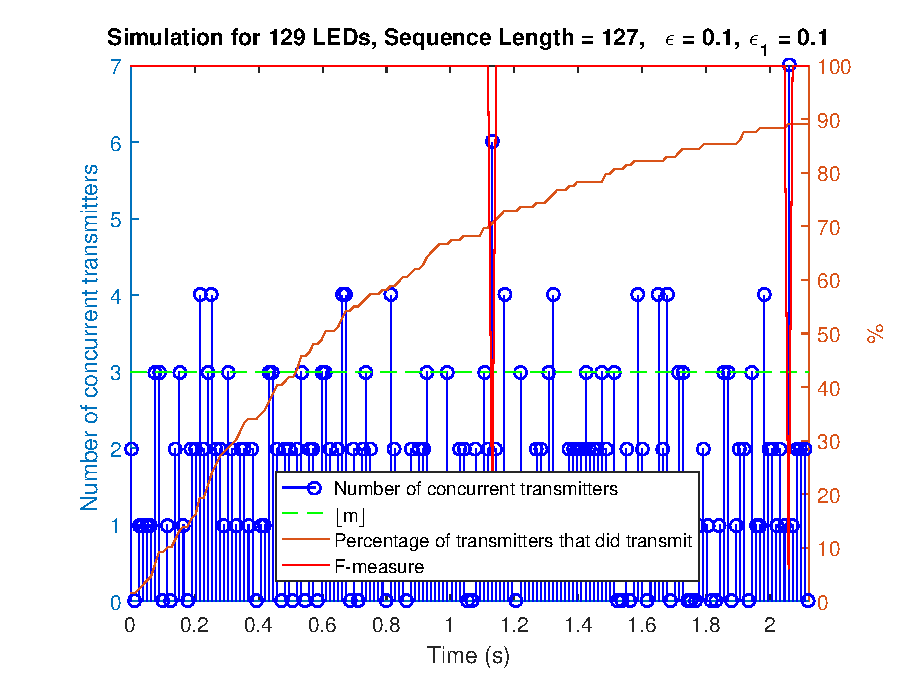
\includegraphics[width=\textwidth]{chapters/evaluation-chapters/simulation/sim-concurrent-tx-and-f-measure-eps=1-n=7.eps}
	\caption{Results of the simulation. Upper plot shows the number of concurrent transmitters per run along with $m$. The lower plot shows the F-measure per run.}
	\label{fig:sim-concurrent-tx-and-f-measure-eps=1-n=7}
\end{figure}

17 \% of the transmitters did not transmit their sequence even once.
This is due to the relatively high value $\epsilon_1 = 0.1$.
There were $k = 84$ runs done.
This results in a time is equal to $\frac{127}{10000} \times 84 = 1.1$ s (See \autoref{eq:time-for-probabilistic-txs}).
So this was a very fast time and pretty accurate, considering that there were only two drops in the F-measure.
But a lot of transmitters did not even transmit once.










The same simulation is done again, but now with $\epsilon = \epsilon_1 = 0.001$.
The plots can be seen in \autoref{sim-concurrent-tx-and-f-measure-eps=001-n=7}.
Note that all transmitters have transmitted at least once.
Only one time the number of concurrent transmitters goes above the $m$ line, but it does not cause interference as shown be the F-measure, which is a constant 1.
So with $\epsilon = \epsilon_1 = 0.001$ it is an accurate setup that can use all the sequences in the set.
But the number of runs is $k = 1023$.
This results in a time of $\frac{127}{10000} \times 1023 = 13.0$ s (See \autoref{eq:time-for-probabilistic-txs}).
This is still a relative small amount of time, but still 13 times larger than the previous simulation.


\begin{figure}[tbp]
	\centering
	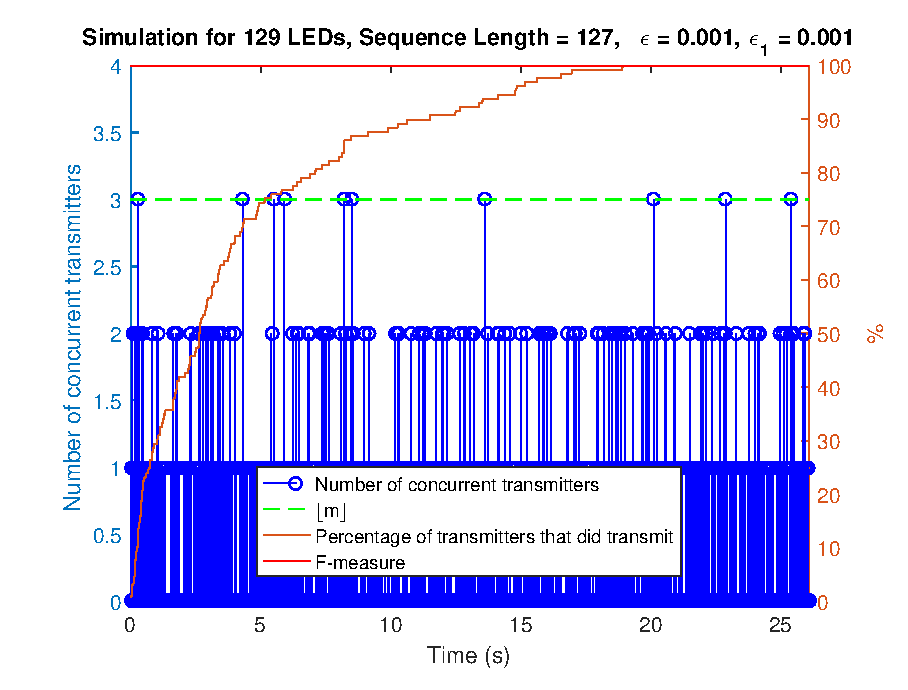
\includegraphics[width=\textwidth]{chapters/evaluation-chapters/simulation/sim-concurrent-tx-and-f-measure-eps=001-n=7.eps}
	\caption{Results of the simulation. Upper plot shows the number of concurrent transmitters per run along with $m$. The lower plot shows the F-measure per run.}
	\label{fig:sim-concurrent-tx-and-f-measure-eps=001-n=7}
\end{figure}



These simulations show that for the probabilistic method there is a clear trade off between time and accuracy.



